\chapter{Introducción}
\label{chapter:introduccion}
\markboth{Introducción}{}
\pagenumbering{arabic}
\setcounter{page}{1}

Antes de comenzar el objeto de estudio de este trabajo, lo primero que debemos hacer es contextualizar el mismo y establecer un marco de trabajo en cuanto a teoría que se empleará en la posterior experimentación y desarrollo del mismo. 

El estudio realizado y plasmado en este trabajo se centra en la obtención de técnicas para la detección de anomalías en conjuntos de datos, concepto que introduciremos posteriormente. En concreto las técnicas que se van a desarrollar son las conocidas como técnicas de ensemble que se basan en el estudio del problema o bien combinando modelos existentes o bien haciendo un estudio pormenorizado aplicando algún criterio por subespacios del conjunto de datos. 

En primer lugar el trabajo desarrollará una introducción a la teoría de aprendizaje y resolución de problemas mediante datos y no por diseño así como la teoría matemática que esto involucra. Esta primera sección nos dará suficiente estructura al trabajo para poder definir en términos de distancias lo que significa que una instancia de un conjunto de datos sea una anomalía.

Posteriormente se desarrollará brevemente algunos conocimientos estadísticos básicos de estadística multivariante para poder introducir el concepto de anomalía desde la perspectiva de las probabilidades condicionadas.

Tras esto podremos entrar en el terreno de la experimentación, desarrollo y explicación de técnicas y puesta en contraste con los algoritmos clásicos para comprobar el desempeño de las nuevas técnicas.

Por último se presentarán las conclusiones obtenidas tras todo este estudio.

\section{Contextualización}

En este contexto y sin haber comenzado la discusión del problema podríamos considerar el establecimiento de una solución al problema de detección de anomalías empleando un algoritmo preciso y óptimo, aunque costoso en tiempo, pero esta solución no es viable en este contexto. Pensemos por un momento en cómo detectar una anomalía en un conjunto de datos. Para poder dar un algoritmo concreto que resuelva siempre el problema de forma óptima tenemos que estar seguros de que somos capaces de definir de forma clara y para todo conjunto de datos cuándo estamos en presencia de un dato anómalo. Pero, ¿sabemos exactamente cuándo sobrepasamos la barrera de dato ligeramente desviado, ruido o una anomalía? 

\begin{figure}[!h]
	\centering
	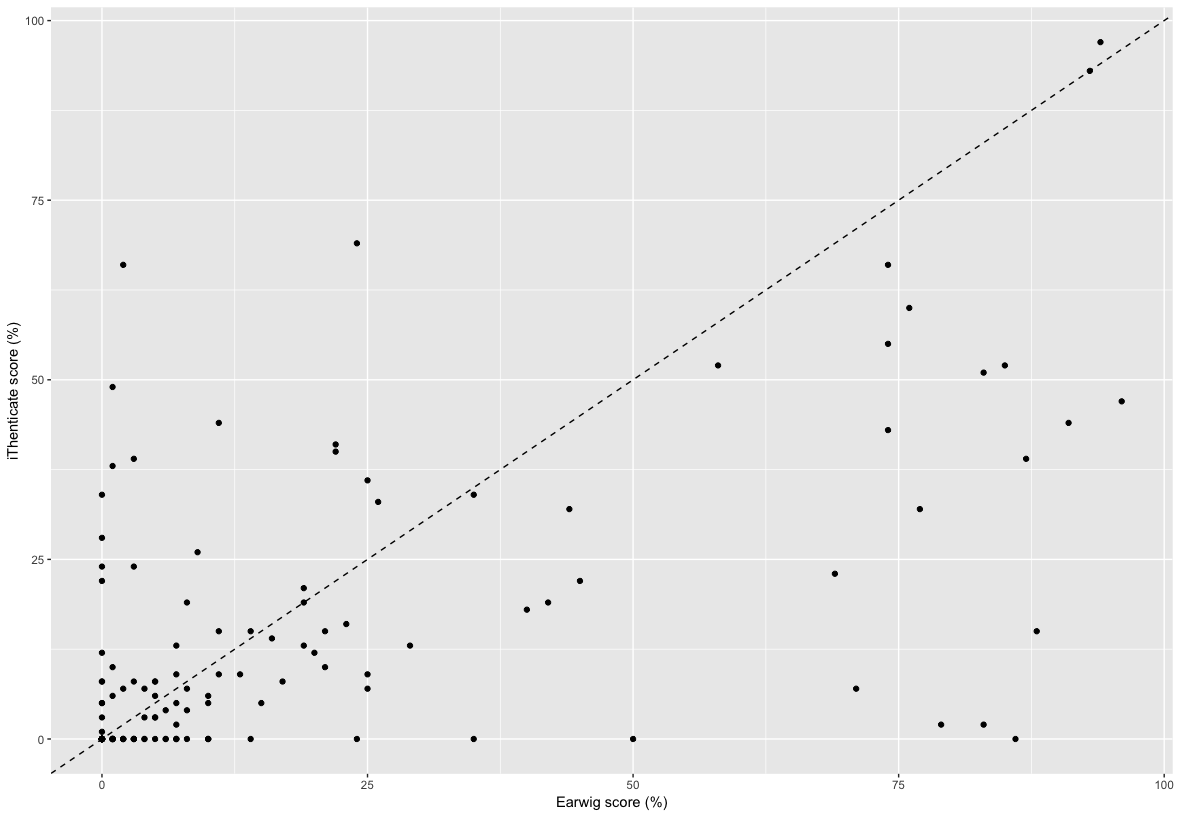
\includegraphics[scale=0.3]{imagenes/1_introduccion}
	\label{1_introduccion}
	\caption{Ejemplo de conjunto de datos \href{https://commons.wikimedia.org/wiki/File:Earwig_ithenticate_scatterplot.png}{(Wikimedia)}}
\end{figure}

Pensemos por ejemplo en este conjunto de datos. Tenemos un clúster muy bien definido en la esquina inferior izquierda y datos dispersos. ¿Podemos afirmar claramente cual es la línea que distingue los datos anómalos de los normales? 

Esta discusión nos lleva a la primera barrera que tenemos que superar en este trabajo. El problema no es resoluble por diseño y por tanto debemos realizar una aproximación a través de los datos. Esto nos va a llevar a aprender de los mismos, valorar cada dato con una puntuación que nos acabará discriminando los datos normales y anómalos.

En el contexto de los problemas resueltos a través de los datos tenemos dos tipos: clasificación y regresión. 

Podríamos pensar que estamos ante un problema de clasificación ordinario, es decir, aprender a través de los datos de entrenamiento cuáles son las anomalías y cuales los datos normales pero no es así. Pensemos que no sabemos ni siquiera nosotros clasificar claramente estas anomalías salvo en algunos ejemplos prácticos. Por ejemplo si le diéramos a una persona un conjunto de datos ya establecido como el que hemos visto anteriormente \ref{1_introduccion} no sería nada fácil e incluso no podemos afirmar que sepamos hacer esta tarea. Por contra si el conjunto de datos es generado en un proceso de trabajo, por ejemplo un conductor de camiones haciendo su ruta, podemos saber cuándo hay una anomalía porque el trabajador la está viviendo y puede señalarla.

Por tanto este problema no es de clasificación al uso pues no es un problema supervisado. Esto significa que, en general no vamos a tener un conjunto etiquetado en el que poder probar cómo aprende nuestro modelo y tendremos que abordar otras técnicas para comprobar el desempeño.

Ahora que comprendemos el alcance del problema podemos intentar profundizar un poco más en la base teórica del mismo analizando las herramientas que el Machine Learning nos provee para abordarlo.

\section{Problema a abordar y técnicas empleadas}

Este estudio va a estar enfocado en el estudio de las anomalías, en concreto, empleando lo que se conocen como técnicas de ensamblaje o algoritmos de ensamblaje. Para ello vamos a dar un marco inicial sobre aprendizaje automático, pues estos algoritmos se basan en los principios de funcionamiento del mismo. 

El objetivo final de esta memoria será la implementación de cinco modelos de ensamblaje: HICS, OUTRES, Trinity, LODA y Mahalanobis Kernel. Estos algoritmos no han sido escogidos al azar, si no con la intención de cubrir el máximo de tipos posibles en cuanto a algoritmos de ensamblaje y sobre todo algoritmos de lo que se suele denominar el estado del arte. Esta expresión es un anglicismo (``state of art'') que no quiere decir más que algoritmos o conocimientos que están a la cabeza en cuanto a rendimiento.

Con estos modelos podremos hacer una comparativa entre lo que se conoce como modelos clásicos y nuestros modelos implementados de ensamblaje, tanto en tiempo como en porcentaje de acierto sobre una serie de conjuntos de datos de los que se dispone información sobre las anomalías.

Con todo esto veremos que hay ideas interesantes en todos los modelos que pueden ser aprovechadas así como los tipos de algoritmos de ensamblaje que resultan ser más exitosos. Esto nos permitirá dar resultados robustos sobre los modelos y además recopilar una serie de ideas que podrían llevar al desarrollo de un modelo original propio que las aglomere.

Para el desarrollo de este trabajo se ha necesitado una base importante de aprendizaje automático. La base teórica de esta rama de la informática y de las matemáticas sustentará el éxito que podemos sacar de los modelos, así como marcar el límite que podemos obtener en cuanto al rendimiento de los mismos. Los modelos están ampliamente basados en técnicas probabilísticas de estadística multivariante por lo que será necesario una introducción de este campo incorporando sobre el temario de la carrera las nociones de vector aleatorio, esperanza condicionada a eventos y $\sigma$-álgebras y probabilidades condicionadas a eventos y $\sigma$-álgebras.

Para la implementación se ha empleado Python creando clases para cada modelo, por lo que se ha utilizado el conocimiento adquirido en asignaturas como Programación y Diseño Orientado a Objetos. Se ha utilizado para el desarrollo la librería NumPy, Sklearn y SciPy así como la librería PyOD que implementa los modelos clásicos de detección de anomalías. 

\section{Contenido básico y fuentes}

El trabajo contiene una primera sección en la que se incluye una introducción de Aprendizaje Automático orientado específicamente a nuestro problema. Para ello primero se hace una contextualización del concepto de aprendizaje así como los principios inductivos que guían el mismo hacia un buen resultado como por ejemplo el ERM o minimización del error empírico. Se aportan también algunas reflexiones y conceptos en cuanto a la aproximación de funciones, que no es más que el objetivo del aprendizaje automático. 

Todos estos conocimientos están basados en la teoría estadística de Vapnik y Chervonenkis que es brevemente repasada y en la que se dan cotas sobre el aprendizaje y su rendimiento. Esta introducción ha sido escrita basándose en tres libros: Learning from Data de Yaser Abu-Mostafa \cite{yaser_learning_2012}, Learning from Data de Cherkassky y Mulier \cite{cherkassky_learning_2007}  y Outlier Ensembles de Aggarwal y Sathe \cite{aggarwal_outlier_2017}.

Este marco nos dirige hacia la primera definición del concepto de anomalía que está basada en distancias y rangos intercuartil que se describen en el libro Outlier Analysis \cite{aggarwal_outlier_2017-1}.

Para dar una definición alternativa y una buena introducción para los modelos debemos hacer una breve introducción estadística. En esta introducción se define un vector aleatorio así como su función de densidad, su función característica y su función de distribución. Se introducen los conceptos de independencia y probabilidad y esperanza condicionada. Por último y aprovechando este contexto se enuncian y demuestran algunas desigualdades y fórmulas famosas. Este contenido viene dado por los apuntes de la asignatura Estadística Multivariante del grado en Matemáticas, los apuntes de la asignatura Procesos Estocásticos del grado en Matemáticas y el libro Probability Theory de M. Loève \cite{m._loeve_probability_1977}.

Tras esto puede ser introducido el concepto probabilístico y basado en densidad de una anomalía. Este concepto viene apoyado en el paper \cite{fabian_keller_hics:_2012} que describe el algoritmo HICS.

Con los dos conceptos de probabilidad y el marco teórico ya planteado se introducen los modelos implementados y el concepto de algoritmos de ensamblaje. Estos conceptos sobre los algoritmos vienen de los libros Outlier Analysis \cite{aggarwal_outlier_2017-1} y Outlier Ensembles \cite{aggarwal_outlier_2017}. Se aporta en esta sección la explicación teórica de cada modelo así como la implementación desarrollada por mí mismo en Python. Los artículos en los que se basa cada algoritmo son \cite{fabian_keller_hics:_2012}, \cite{aggarwal_outlier_2017}, \cite{pevny_loda:_2016} y \cite{muller_statistical_2011}.

Finalmente se analiza el comportamiento de todos los modelos en la sección de resultados frente a los algoritmos considerados como clásicos. Se aportan conclusiones tras todo el trabajo y, al haber margen de mejora, se aportan algunas ideas que podrían aplicarse en un futuro para desarrollar un modelo propio.

\section{Objetivos}

Por todo lo descrito anteriormente el trabajo tiene los siguientes objetivos claros:

\begin{itemize}
	\item Desarrollar un marco teórico sobre el aprendizaje en problemas de clasificación y problemas no supervisados o semi-supervisados.
	\item Estudiar el estado del arte de los algoritmos de ensamblaje.
	\item Estudiar la teoría estadística que rodea los algoritmos de ensamblaje.
	\item Entender los fundamentos teóricos y el funcionamiento de los modelos implementados.
	\item Desarrollar una implementación de los modelos.
	\item Obtener una comparativa entre los modelos clásicos y los de ensamblaje.
\end{itemize}

Todos estos objetivos han sido alcanzados en el desarrollo de este estudio, obteniendo además algunas ideas nuevas que pudieran ser la base de un modelo propio.